\documentclass[UTF8,titlepage,a4paper]{ctexart}
\usepackage{amsmath,amssymb,amsthm,amsfonts,amscd}
\usepackage{fontspec}
\setmainfont{Times New Roman}
\usepackage{graphicx}
\usepackage{titlesec}
\usepackage{makecell}
\usepackage{longtable}
\usepackage{xcolor}
\usepackage{tcolorbox}
\usepackage{soul}
\usepackage{adjustbox}
\usepackage{tcolorbox}
\usepackage{enumerate}
\usepackage{pdfpages}
\usepackage{float}
\usepackage{colortbl}
\usepackage{tabularx}
\usepackage{multirow}
\usepackage{pgfplots}
\usepackage{hyperref}
\usepackage{booktabs} % For better looking tables

\numberwithin{figure}{section}
\usepackage[left=1.25in,right=1.25in,%
top=1in,bottom=1in]{geometry}
\usepackage{color}
\titleformat{\section}
  {\raggedright\LARGE\bfseries}{\thesection}{1em}{}
\begin{document}
\title{模电报告}
\author{赵伯远}
\date{\today}
\thispagestyle{empty}
\begin{center}
{\fontsize{30pt}{21pt}\selectfont \textbf{东华大学课程设计报告}}

\vspace{10cm}

\begin{tabular}{l}
    {\large 课程名称:电子技术设计与实践(数电)} \\
    \\
    \large{课题名称:\underline{\hspace{58pt}数字频率计\hspace{58pt}}}  \\
    \\
    \large{指导教师:\underline{\hspace{70pt}宫晓蕙\hspace{70pt}}} \\
    \\
    \large{学生姓名:\underline{\hspace{70pt}赵伯远\hspace{70pt}}} \\
    \\
    \large{学生班级学号:\underline{\hspace{11pt}人工智能2101 211440128\hspace{11pt}}} \\
    \end{tabular}
\end{center}
\clearpage
\setcounter{page}{1}
\tableofcontents
\clearpage

\section{设计指标}

在本项目中,的目标是设计和实现一个测量 TTL 方波信号频率的数字系统。用按键选择测量信号频率。测量值采用 4 个 LED 七段数码管显示。下面是设定的主要设计指标:

\subsection{设计指标}
\begin{itemize}
    \item 频率范围:100.0 Hz 到 999.9 MHz
    \item 精度:±0.1\%
    \item 分辨率:0.1 Hz
\end{itemize}

\section{系统概述}

\subsection{设计思想}

数字频率计的设计理念基于现代数字技术的高度集成和精确性。为了确保准确、稳定的频率测量,选择了间接计数法。这种方法通过在固定时间间隔内计算脉冲数量来测量频率,从而避免了直接测量高频信号所带来的挑战。此外,考虑到现代数字技术的进步,还采用了高精度的时基和计数器,以进一步提高测量的准确性。

\subsection{可行性论证}

在现代的电子技术背景下,利用数字技术实现频率计是完全可行的。数字技术,特别是高度集成的数字ICs,为提供了创建高度精确、稳定且功能丰富的设备的机会。此外,与传统的模拟技术相比,数字技术还提供了更好的噪声容限、更低的功耗和更小的尺寸。

\subsection{各功能的组成}

数字频率计的核心组成部分包括:

\begin{enumerate}
    \item \textbf{输入放大器和调节器}:这部分确保输入信号达到适当的幅度和形状,以供后续电路处理。
    \item \textbf{门控时间基准电路}:它为计数器提供一个固定的时间窗口,确保每次测量都在相同的时间间隔内进行。
    \item \textbf{计数器}:这是系统的核心,负责在给定的时间窗口内计算脉冲数量。
    \item \textbf{显示器}:将计数器的输出转换为用户可读的频率值,并在LED数码管上显示。
\end{enumerate}

\subsection{总体工作过程}

当信号进入频率计时,它首先通过输入放大器和调节器进行初步处理。调整后的信号随后进入计数器,在一个由门控时间基准电路定义的固定时间窗口内被计数。计数结束后,计数器的输出传送到显示器,并转换为相应的频率值显示出来。

示意图如下:

\begin{figure}[H]
\centering
 \resizebox{1\textwidth}{!}{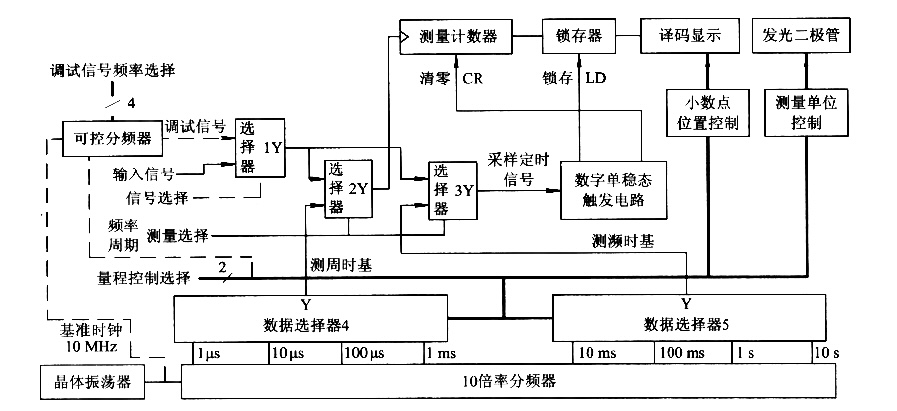
\includegraphics{./img_de/flowchart.jpg}}
 \caption{设计流程图}
 \label{}
\end{figure}

\clearpage
\section{单元电路设计与分析}

\subsection{10 倍率分频器}

\begin{enumerate}
    \item \textbf{7490 二进制计数器概述}:
    
    7490是一个四位二进制计数器,其工作原理基于异步计数机制。它有四个输出:QA, QB, QC, 和 QD,分别代表$2^0$, $2^1$, $2^2$, 和 $2^3$的权值。此外,它还配备了异步清零和预设功能。
    
    \item \textbf{分频原理}:
    
    由于7490是一个十进制计数器,因此当它从0计数到9后,它会溢出并返回到0。当这一溢出事件发生时,它可以驱动下一个计数器,使其加1。通过这种方法,前一个计数器的QD输出与后续计数器的时钟输入相连接,从而实现串联计数。
    
    \item \textbf{电路分析}:
    
    在所提供的电路中,有8个串联的7490计数器。输入频率为10MHz的信号首先被第一个7490计数器接收。由于每个7490的分频比是10:1,经过四个串联的计数器后,输出频率将是原始频率的$10^{-8}$倍,即0.1Hz。
    
    \item \textbf{同步与异步操作}:
    
    尽管7490基于异步计数原理,但其设计中的“清零”功能允许工程师在必要时对所有计数器进行同步复位。这确保了在给定的时间点,所有计数器都从已知的初始状态开始操作。
\begin{figure}[H]
\centering
 \resizebox{1\textwidth}{!}{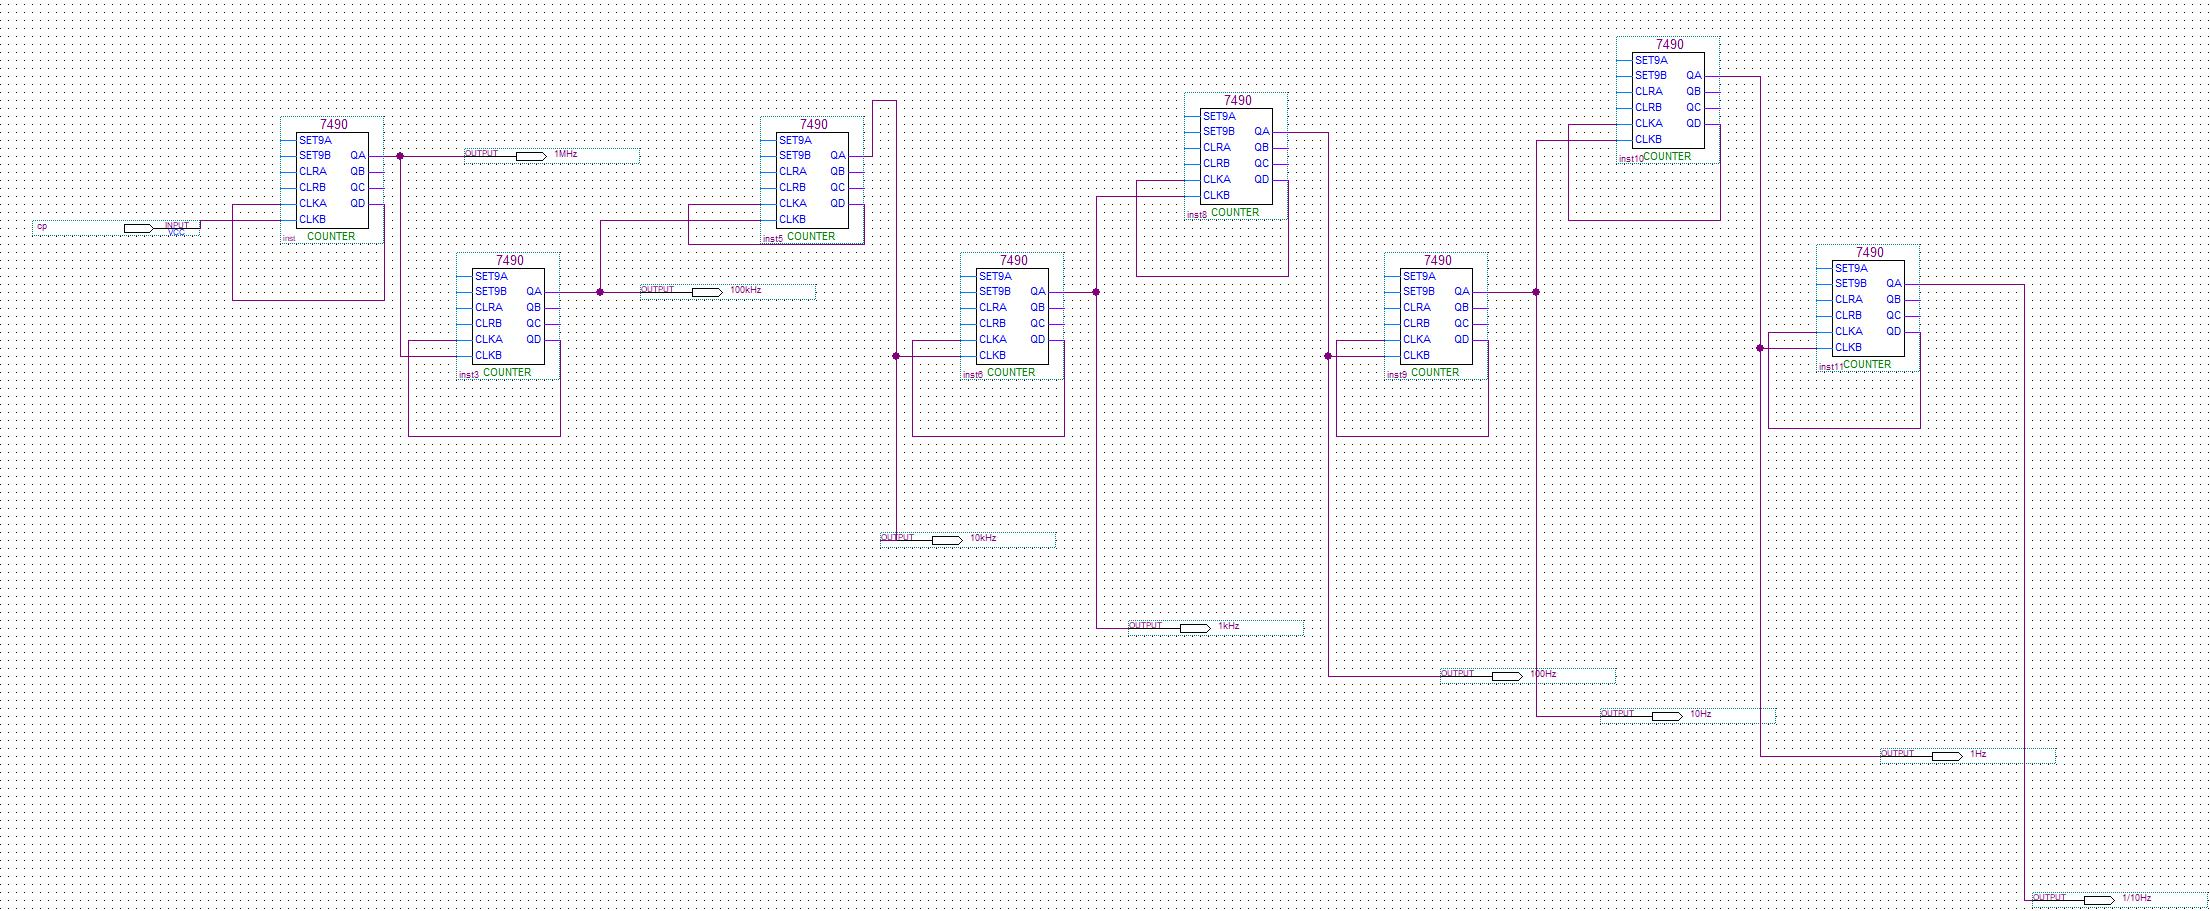
\includegraphics{./img_de/fpq.jpg}}
 \caption{10 倍率分频器}
 \label{}
\end{figure}
\end{enumerate}
\begin{figure}[H]
    \centering
     \resizebox{0.5\textwidth}{!}{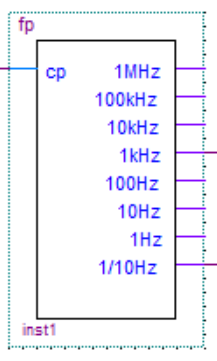
\includegraphics{./img_de/fpq_fz.png}}
     \caption{封装后结果}
     \label{}
    \end{figure}
\subsection{译码显示电路}


\begin{enumerate}
    \item \textbf{主要组件}:
    \begin{enumerate}
        \item \textbf{74153M}:这是一个双4线-1线数据选择器/多路选择器。在此设计中,有多个此类选择器,其主要功能是从多个输入中选择一个,并将其传递到输出。
        
        \item \textbf{74160}:一个十进制的同步计数器,它能够同步地对输入脉冲进行计数。当它从0计数到9后,它会回到0并输出一个脉冲。
    \end{enumerate}

    \item \textbf{工作原理}:
    \begin{enumerate}
        \item \textbf{译码}:电路的输入数据(例如`d0`至`d3`)经过74153M多路选择器进行选择性地传递。
        
        \item \textbf{计数}:74160计数器从1MHz开始计数。每次达到10时,它都会溢出并通过`RCO`端口输出一个脉冲。此脉冲可以用来驱动另一个级联的计数器。
        
        \item \textbf{7seg电路转换}:此部分电路的功能是将数字逻辑值转换为七段显示数码管可以识别的信号。这使得数字逻辑值可以直接显示在七段数码管上。
    \end{enumerate}

    \item \textbf{分频功能}:
        电路右侧的频率列表从1MHz开始递减。这表明计数器与多路选择器结合使用,实现分频功能,从而将1MHz的输入频率减少到更低的频率,如10kHz、1kHz等。
    
    \item \textbf{输出信号与显示}:
     设计中的数字信号通过7seg转换电路,最终被转换为`a`至`g`的七段信号,这些信号驱动七段显示数码管,从而显示相应的数字。

    \item \textbf{地线连接}:
     所有的集成电路都连接到公共地线,确保整个电路有一个共同的电压参考点。
     \begin{figure}[H]
     \centering
      \resizebox{1\textwidth}{!}{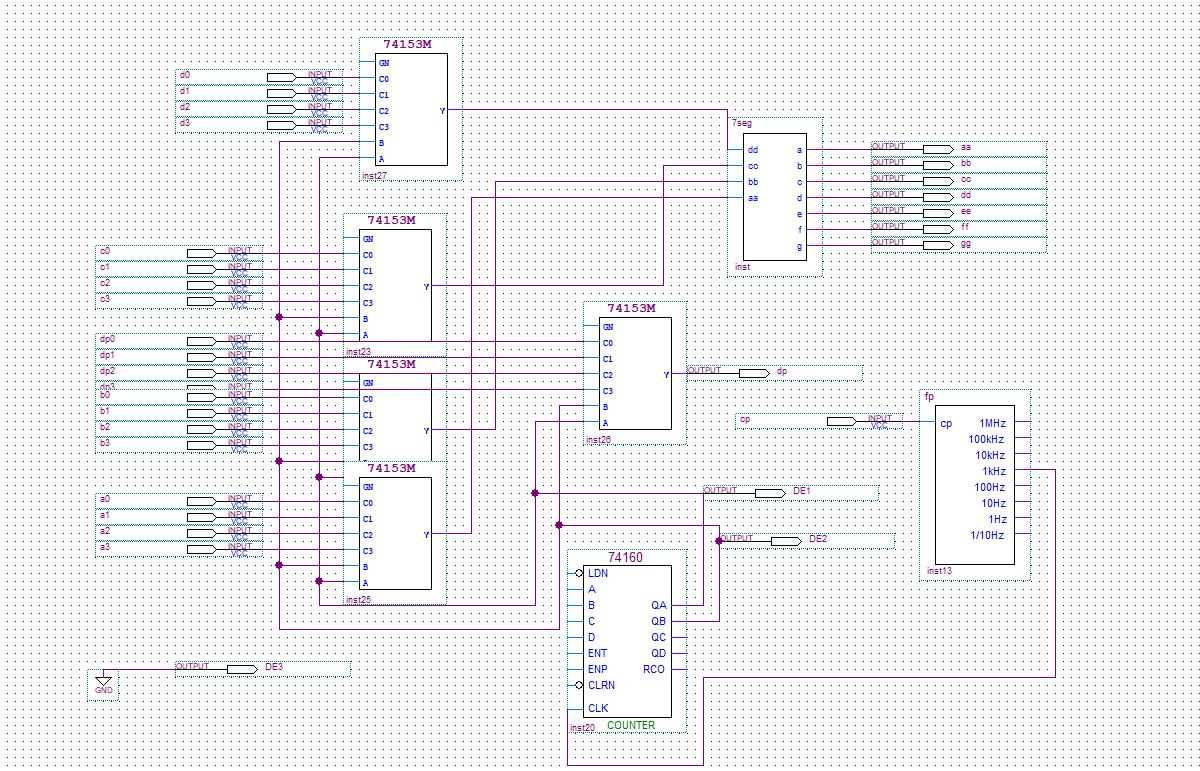
\includegraphics{./img_de/ymxs.jpg}}
      \caption{译码显示电路}
      \label{}
     \end{figure}
     \begin{figure}[H]
     \centering
      \resizebox{0.5\textwidth}{!}{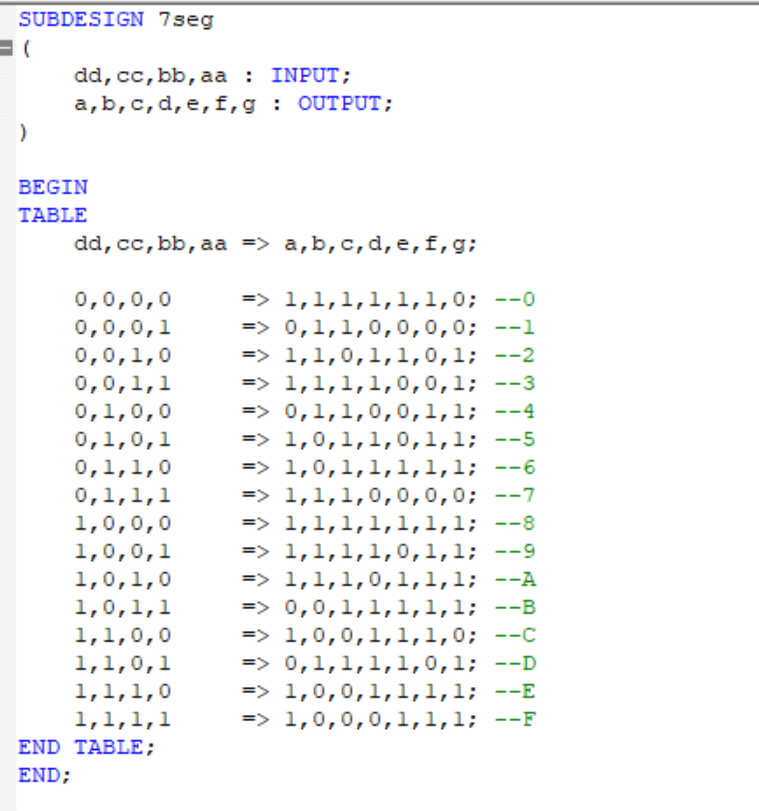
\includegraphics{./img_de/7seg.png}}
      \caption{7段译码显示}
      \label{}
     \end{figure}
     \begin{figure}[H]
     \centering
      \resizebox{0.5\textwidth}{!}{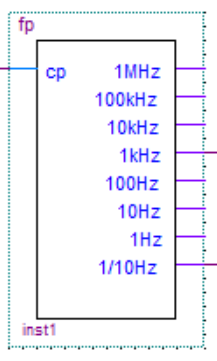
\includegraphics{./img_de/ymxs_fz.png}}
      \caption{封装后结果}
      \label{}
     \end{figure}
\end{enumerate}

\subsection{单稳态触发电路}

\begin{enumerate}
    \item \textbf{主要组件及其功能}:
    \begin{enumerate}
        \item \textbf{触发器}:这些触发器(例如`inst1`, `inst2`, `inst8`)主要用作存储元件。它们在接收到特定的输入信号时将其输出状态改变。
        
        \item \textbf{逻辑门}:这些门(例如`AND2`和`NOR`)用于处理、组合和产生逻辑信号。
    \end{enumerate}
    
    \item \textbf{工作原理}:
    \begin{enumerate}
        \item \textbf{时基信号生成}:当输入`M`和`CP`同时变为高电平时,`inst1`和`inst2`触发器被设置为高电平。随后,通过逻辑门进行处理,产生一个短暂的脉冲,这个脉冲用于驱动`2Gate`。
        
        \item \textbf{显示锁存}:通过`2Gate`的输出,当D触发器的输出为高电平时,它将允许显示信号通过,实现了显示锁存的功能。
        
        \item \textbf{计数清零}:`inst3`触发器的输出被用作清零信号(`2CLR`)。当它为高电平时,它将使下游设备的计数值清零。设计时发现非门的延迟并不稳定,故使用D触发器代替, 使得稳定延迟半个cp周期, 保证清零发生在锁存之后。
    \end{enumerate}
    
    \item \textbf{单稳态特性}:
    
    当电路从稳定状态被一个外部信号触发时,它会短暂地进入另一个状态,然后自动返回到其初始状态。这种行为特征是由`inst1`和`inst2`触发器之间的相互连接实现的。

    \item \textbf{输出信号}:

    主要的输出信号是`2Gate`的输出和`2CLR`。这些信号可以进一步连接到其他电路或显示设备,实现所需的功能。
    \begin{figure}[H]
    \centering
     \resizebox{1\textwidth}{!}{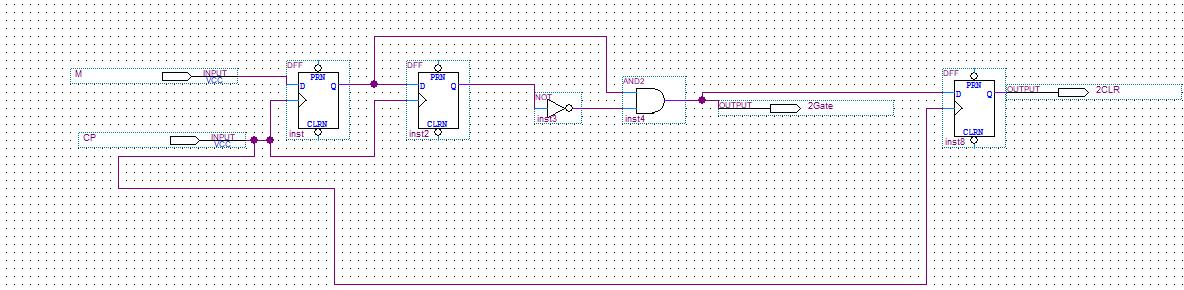
\includegraphics{./img_de/dwtcf.jpg}}
     \caption{单稳态触发电路}
     \label{}
    \end{figure}
    \begin{figure}[H]
    \centering
     \resizebox{0.5\textwidth}{!}{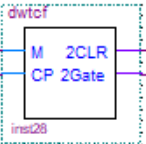
\includegraphics{./img_de/dwtcf_fz.png}}
     \caption{封装后结果}
     \label{}
    \end{figure}
\end{enumerate}

\subsection{调试信号发生器}
\begin{enumerate}
    \item \textbf{主要组件及其功能}:
    \begin{enumerate}
        \item \textbf{逻辑门}:该电路中的NOT逻辑门用于信号的逻辑反转。
        
        \item \textbf{74160计数器}:这是一个8位同步计数器,用于生成序列信号。它可以根据输入条件进行计数,并产生相应的输出。
    \end{enumerate}
    
    \item \textbf{工作原理}:
    \begin{enumerate}
        \item \textbf{输入信号}:`A[0:1]`, `B[0:1]`,  `C[0:1]`,`D[0:1]` 是电路的输入信号, 用按键进行控制,用于设置计数器的初始状态, 以达到不同的分频效果。
        
        \item \textbf{计数操作}:当`CLK`信号上升沿到来时,74160计数器开始计数。计数器的计数值可以通过`QA`到`QD`的输出观察。`RCO`是一个进位输出,当计数器达到最大值并回绕时,它会产生一个输出脉冲。
        
        \item \textbf{加载和清零功能}:`LDN`信号用于从`A`到`D`的输入加载一个值到计数器。`CLR`信号用于异步清零计数器。
        
        \item \textbf{使能控制}:`ENT`和`ENP`是计数器的使能端,当它们被激活时,计数器开始工作。
    \end{enumerate}
    
    \item \textbf{工作流程分析}:
    当为计数器提供`0110`作为输入值:
    \begin{enumerate}
        \item 计数器通过`LDN`信号加载输入值`0110`。
        
        \item 当`CLK`信号上升沿到来,并且`ENT`和`ENP`都为高电平时,计数器从其当前值(这里是`0110`)开始计数。
        
        \item 计数器每次上升沿递增1,直到它达到`1111`。当它数到`1111`并尝试再递增时,它将回到`0000`并输出一个`RCO`脉冲。
        
        \item 因此,每4个`CLK`上升沿,都会得到一个`RCO`脉冲输出,实现了4分频的功能。
    \end{enumerate}
    
    预置数与分频比的关系如下:
    
\begin{table}[h]
    \centering
    \begin{tabular}{|c|c|c|}
    \hline
    分频数N & 预置数 (ABCD) & 理论频率 (Hz) \\
    \hline
    2 & 0001 & 500.0 \\
    3 & 1110 & 333.3 \\
    4 & 0110 & 250.0 \\
    5 & 1010 & 200.0 \\
    6 & 0010 & 166.7 \\
    7 & 1100 & 142.9 \\
    8 & 0100 & 125.0 \\
    9 & 1000 & 111.1 \\
    10 & 0000 & 100.0 \\
    \hline
    \end{tabular}
    \caption{分频数与预置数的对应关系}
    \end{table}
    
    \item \textbf{输出信号}:
    \begin{enumerate}
        \item 主要的输出信号是`QA`到`QD`,表示计数器的当前状态。此外,`RCO`表示计数器的进位输出。
        
        \item `Q out`是电路的总输出,可能用于驱动其他电路或作为信号发生器的输出。
    \end{enumerate}

    \item \textbf{应用场景}:

    该调试信号发生器可以用于产生特定的信号模式,用于测试其他数字系统。

    \begin{figure}[H]
    \centering
     \resizebox{1\textwidth}{!}{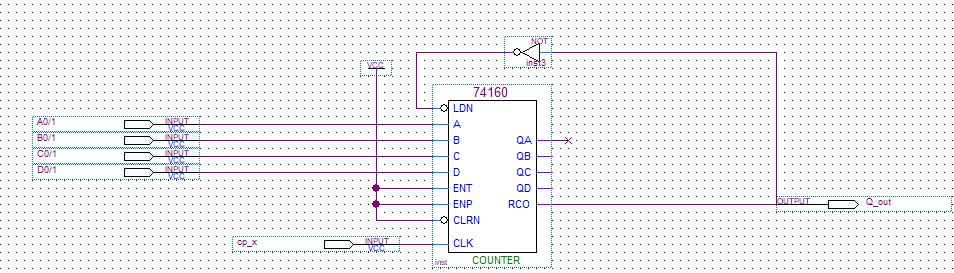
\includegraphics{./img_de/debug_signal.jpg}}
     \caption{调试信号发生器}
     \label{}
    \end{figure}
    \begin{figure}[H]
    \centering
     \resizebox{0.5\textwidth}{!}{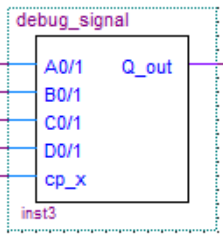
\includegraphics{./img_de/debug_signal_fz.png}}
     \caption{封装后结果}
     \label{}
    \end{figure}

\end{enumerate}

\subsection{数字频率计}

数字频率计主要包括四个核心部分:

\begin{enumerate}
    \item \textbf{预分频器}:
    
    该部分接收高频的输入信号,并通过计数器或触发器将其分频,使其频率降低至后续计数电路可以处理的范围内。
    
    \item \textbf{计数器}:
    \begin{itemize}
        \item 电路中存在多个串联的计数器,它们从预分频器接收降频后的信号并开始计数。
        \item 使用一个单稳态电路来产生一个固定的门时间。在此时间间隔结束时,计数器的值代表了输入信号在该时间窗口内的脉冲数,从而得出输入信号的频率。
    \end{itemize}
    
    \item \textbf{显示锁存与译码}:
    \begin{itemize}
        \item 为了保持显示的稳定性并避免数字在变化时的闪烁,使用74374八位触发器对输出进行锁存。
        \item 译码器将计数器的输出从二进制形式转换为七段显示器可显示的形式。每个计数器的输出都连接到一个译码器,确保频率的每一位数字都能正确显示。
    \end{itemize}
    
    \item \textbf{显示输出}:
    
    最终的显示格式为xxx.x,包括三位整数和一位小数,以及小数点,使得测量结果易于读取和解释。

    \begin{figure}[H]
    \centering
     \resizebox{1\textwidth}{!}{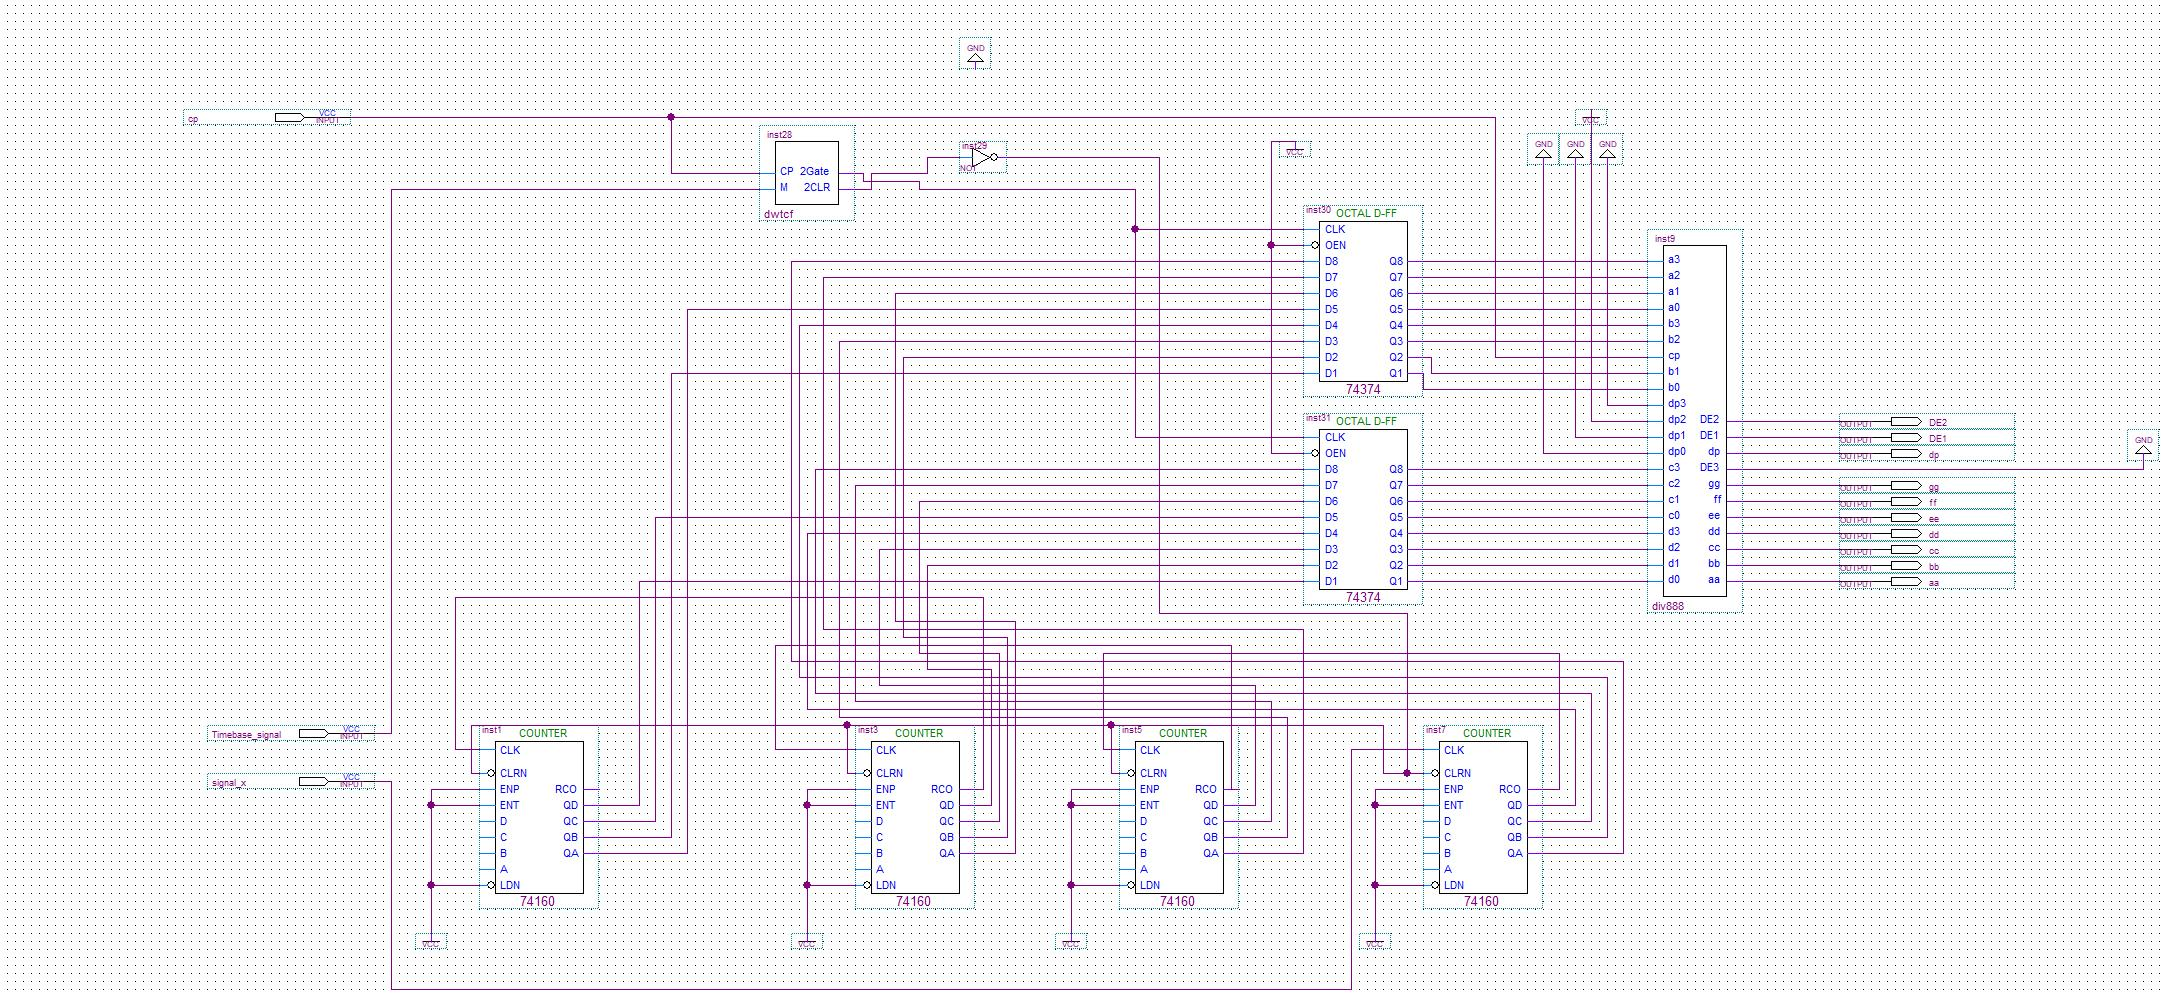
\includegraphics{./img_de/test.jpg}}
     \caption{数字频率计}
     \label{}
    \end{figure}
    \begin{figure}[H]
    \centering
     \resizebox{0.5\textwidth}{!}{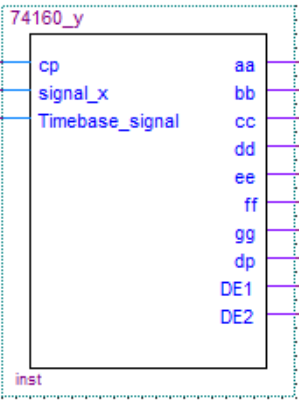
\includegraphics{./img_de/test_fz.png}}
     \caption{封装后结果}
     \label{}
    \end{figure}
\end{enumerate}

\subsection{电路总图}
整体实验电路图如下:
\begin{figure}[H]
\centering
 \resizebox{1\textwidth}{!}{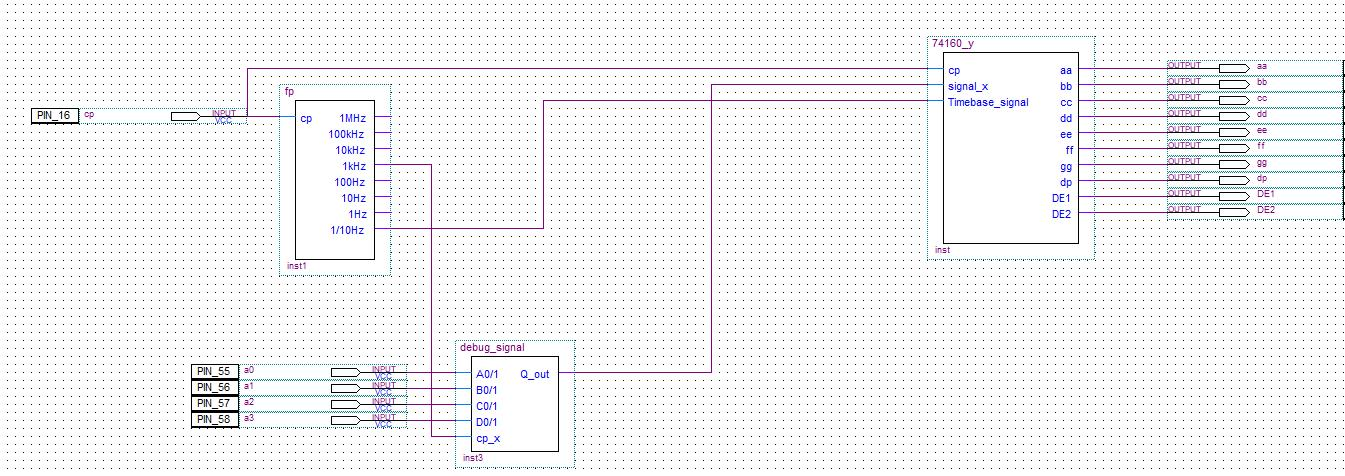
\includegraphics{./img_de/final.jpg}}
 \caption{电路总图}
 \label{}
\end{figure}

\clearpage
\section{电路的组构与调试}
\subsection{测试故障分析与排除}
\begin{enumerate}
    \item Q1: 电路无法正常工作,七段数码管只显示一个。
    
    A: 故障为cp输入没有正确接入,且在电路图中被其他元件覆盖,重构元件后发现并解决。

    \item Q2: 测试信号没有正确分频,具体而言,当D=1时无法测得正确的频率。
    
    A: 故障为输出端接在了QD上,导致分频不正确,改接到RCO上后解决。

    \item Q3: 电路过于繁杂,不利于调试
    
    A: 尽可能封装电路,并分块调试,最终效果如电路总图所示
\end{enumerate}

\subsection{功能的测试方法、步骤、设备}
\begin{enumerate}
    \item \textbf{功能测试的方法}:
    \begin{enumerate}
        \item SWA, SWB, SWC, SWD表示产生不同调试信号。
        \item 4 个 LED 七段数码管,显示测量结果。
    \end{enumerate}
    
    \item \textbf{功能测试的步骤}:
    \begin{enumerate}
        \item 全编译 Compile。
        \item 下载 Programmer。
        \begin{itemize}
            \item 通过下载电缆将编程文件下载到器件中。
            \item 用下载电缆将 PC 机与实验设备相连,实验装置打开电源,在 Tools 菜单中选择 Programmer,设置下载电缆为 ByteBlaste[LPT1]、选择下载模式为 JTAG,然后加载要下载的*.sof 文件,注意 Device 栏是否为选择的器件,然后点击 Start 开始下载。完成编程后芯片即能实现所设计的逻辑功能。
            \item LP-2900 实验装置绿灯亮,开始测试。
        \end{itemize}
    \end{enumerate}
    
    \item \textbf{功能测试的设备}:
    \begin{enumerate}
        \item Quartus 软件。
        \item LP-2900 实验装置。
    \end{enumerate}
\end{enumerate}

\clearpage
\subsection{功能测试结果}
功能测试结果记录如下:
\begin{table}[h]
    \centering
    \begin{tabular}{|c|c|c|c|}
    \hline
    分频数N & 预置数 (ABCD) & 理论频率 (Hz) & 实测频率 (Hz) \\
    \hline
    2 & 0001 & 500.0 & 500.0 \\
    3 & 1110 & 333.3 & 333.3 \\
    4 & 0110 & 250.0 & 250.0 \\
    5 & 1010 & 200.0 & 200.0 \\
    6 & 0010 & 166.7 & 166.7 \\
    7 & 1100 & 142.9 & 142.8 \\
    8 & 0100 & 125.0 & 125.0 \\
    9 & 1000 & 111.1 & 111.1 \\
    10 & 0000 & 100.0 & 100.0 \\
    \hline
    \end{tabular}
    \caption{实验数据}
\end{table}

实验图见附录。

\clearpage
\section{结束语}
\subsection{对设计题目的结论性意见及进一步改进的意向说明}
在本次课程设计中,我使用LP-2900实验装置制作了数字频率计,通过这一实践过程,我认为此设计题目非常具有实际应用价值和教育意义。它不仅让我实际接触并应用了数字电路的基本理论,而且也帮助我加深了对数字逻辑设计的认识。

尽管当前的设计已经可以满足基本的功能需求,但我认为还有以下几点可以进一步改进和完善:
\begin{enumerate}
    \item \textbf{显示界面优化}:目前的显示是基于LED七段数码管的,未来可以考虑使用液晶显示屏,使得数据显示更为直观和美观。
    \item \textbf{增加更多功能}:可以考虑增加保存功能,以便于保存测量到的频率数据,或者设计一个数据传输功能,使得数据可以直接传输到计算机或其他设备上。
    \item \textbf{提高测量精度}:虽然当前的频率计设计已经具有较好的测量精度,但总是有提高的空间。可以考虑引入更先进的计数器和传感器,以提高测量的准确性。
\end{enumerate}

\subsection{总结收获}
通过这次数字频率计的设计与制作,我深深地感受到了理论知识与实际操作之间的紧密联系。

首先,这次设计锻炼了我的实际操作能力和实验技巧。在设计过程中,我不仅需要运用所学的数字电路理论知识,还需要面对并解决各种实际问题,这使我对数字电路有了更深入的了解。

更重要的是,我深刻地认识到了不断探索和学习的重要性。在设计中,我遇到了很多之前没有遇到过的问题,通过查阅资料、咨询老师和与同学讨论,我不断地克服了这些困难。这使我明白了,作为一个工程师,持续的学习和进步是非常重要的。

总之,这次课程设计为我提供了一个宝贵的实践机会,使我收获颇丰,对我的未来学习和工作都有很大的帮助。

\section*{参考文献}

[1]赵曙光.数字电路及系统设计.北京:高等教育出版社,2011

[2]崔葛瑾.基于 FPGA 的数字电路系统设计.西安:西安电子科技大学出版社,2008.7

\clearpage

\section*{附录1: 电路总图}
\begin{figure}[H]
\centering
 \resizebox{1\textwidth}{!}{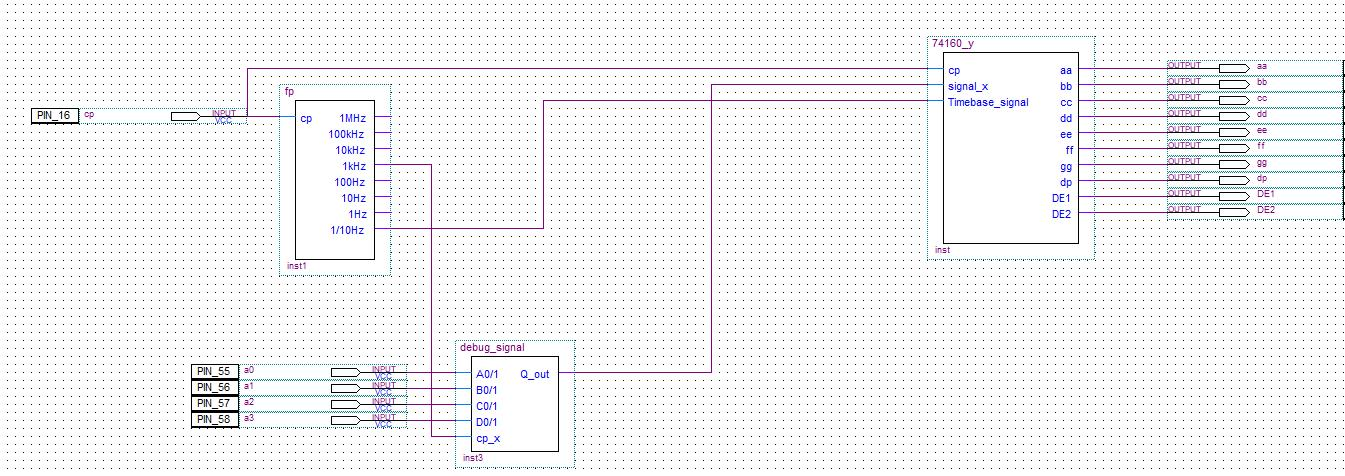
\includegraphics{./img_de/final.jpg}}
 \caption{电路总图}
 \label{}
\end{figure}

\section*{附录2: 功能测试结果图}

\begin{figure}[H]
\centering
 \resizebox{0.75\textwidth}{!}{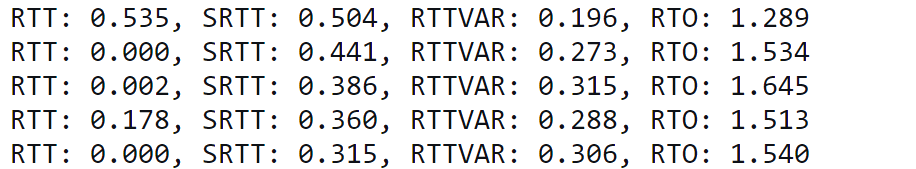
\includegraphics[angle=0]{./img_de/result/2.jpg}}
 \caption{分频数为2时的测试结果}
 \label{}
\end{figure}

\begin{figure}[H]
\centering
 \resizebox{0.75\textwidth}{!}{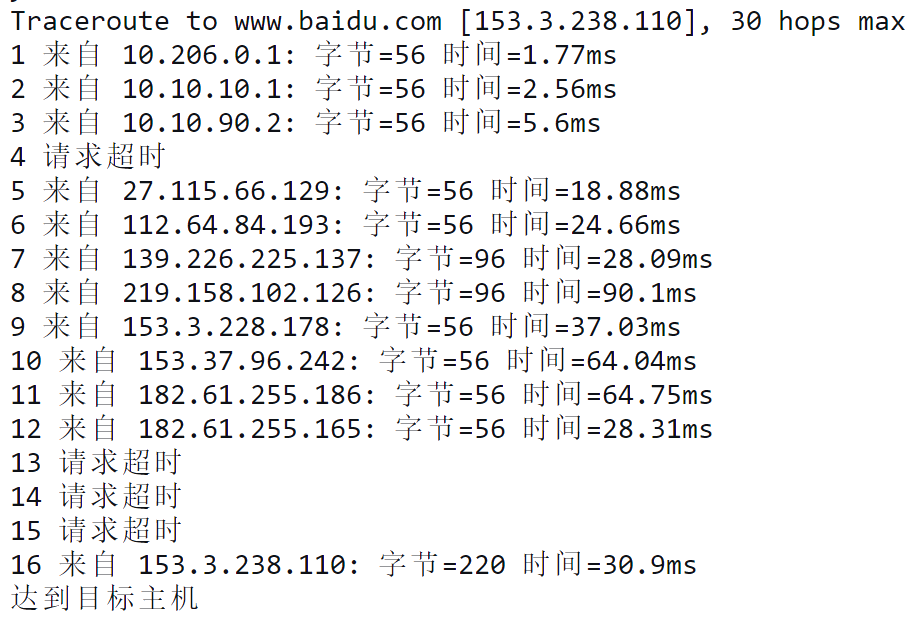
\includegraphics[angle=0]{./img_de/result/3.jpg}}
 \caption{分频数为3时的测试结果}
 \label{}
\end{figure}

\begin{figure}[H]
\centering
 \resizebox{0.75\textwidth}{!}{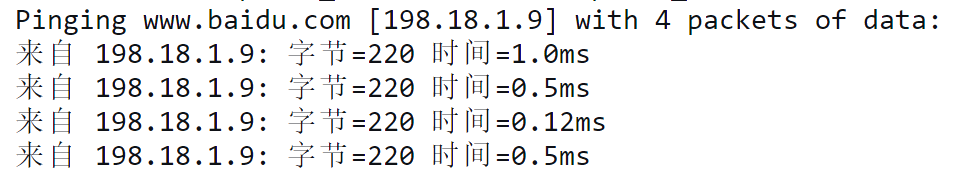
\includegraphics[angle=0]{./img_de/result/4.jpg}}
 \caption{分频数为4时的测试结果}
 \label{}
\end{figure}

\begin{figure}[H]
\centering
 \resizebox{0.75\textwidth}{!}{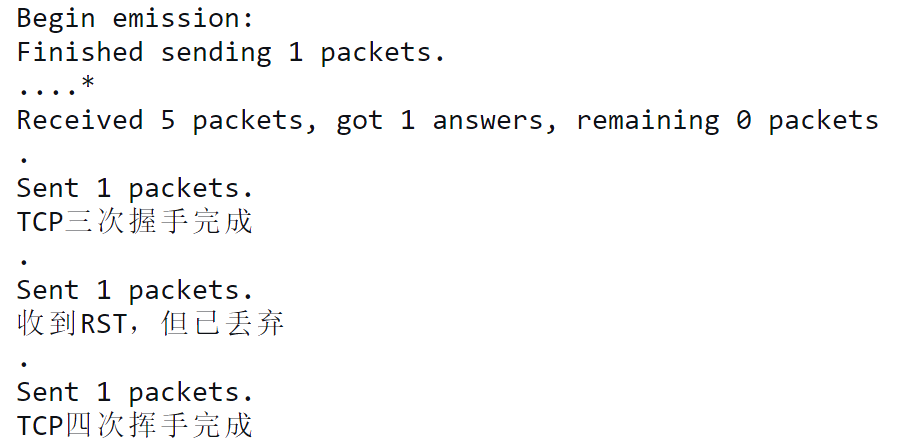
\includegraphics[angle=0]{./img_de/result/5.jpg}}
 \caption{分频数为5时的测试结果}
 \label{}
\end{figure}

\begin{figure}[H]
\centering
 \resizebox{0.75\textwidth}{!}{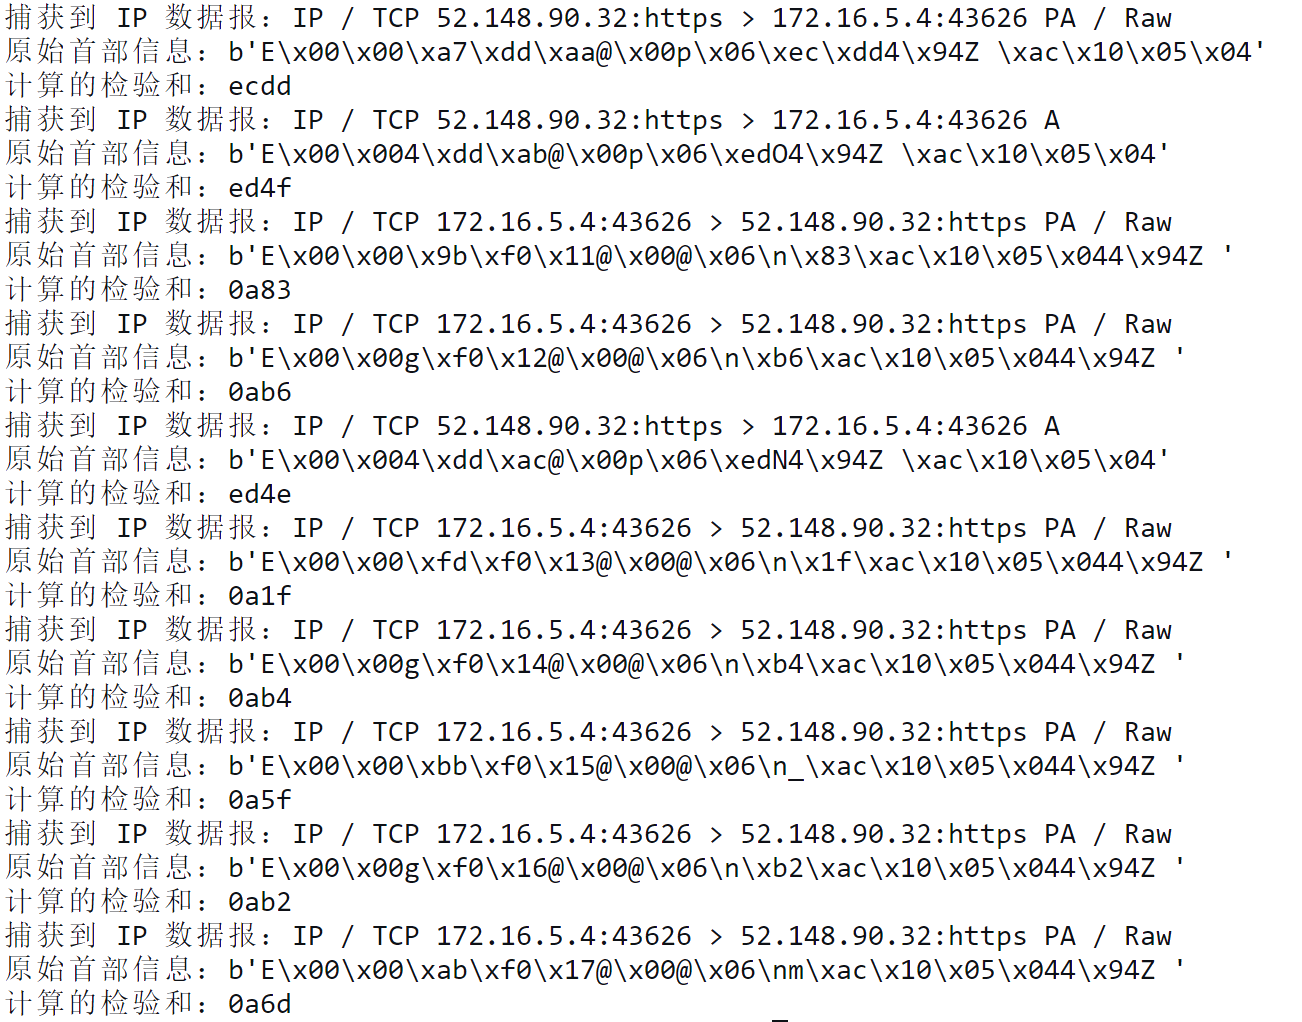
\includegraphics[angle=0]{./img_de/result/6.jpg}}
 \caption{分频数为6时的测试结果}
 \label{}
\end{figure}

\begin{figure}[H]
\centering
 \resizebox{0.75\textwidth}{!}{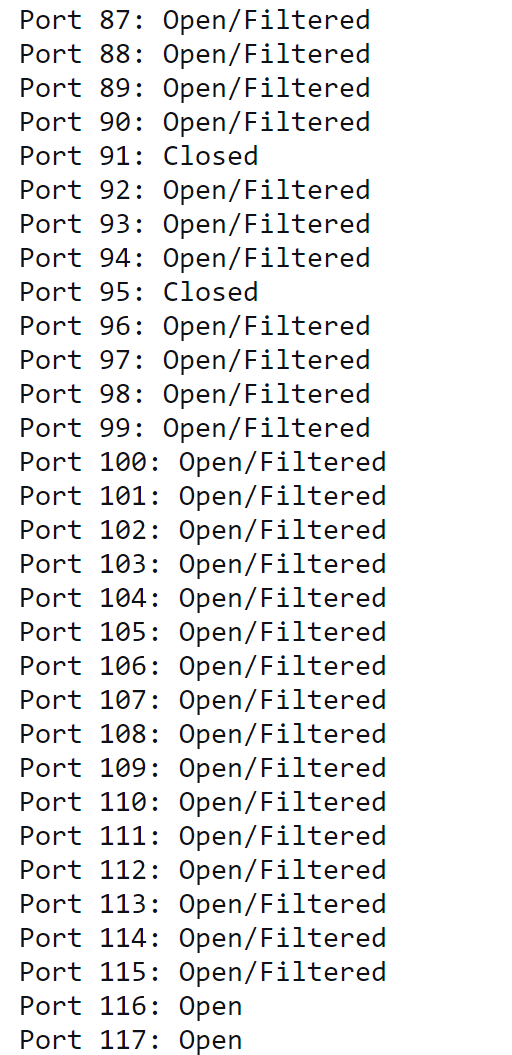
\includegraphics[angle=0]{./img_de/result/7.jpg}}
 \caption{分频数为7时的测试结果}
 \label{}
\end{figure}

\begin{figure}[H]
\centering
 \resizebox{0.75\textwidth}{!}{\includegraphics[angle=0]{./img_de/result/8.jpg}}
 \caption{分频数为8时的测试结果}
 \label{}
\end{figure}

\begin{figure}[H]
\centering
 \resizebox{0.75\textwidth}{!}{\includegraphics[angle=0]{./img_de/result/9.jpg}}
 \caption{分频数为9时的测试结果}
 \label{}
\end{figure}

\begin{figure}[H]
\centering
 \resizebox{0.75\textwidth}{!}{\includegraphics[angle=0]{./img_de/result/10.jpg}}
 \caption{分频数为10时的测试结果}
 \label{}
\end{figure}



\end{document}

